\documentclass[a4paper,12pt,preview]{report} %размер бумаги устанавливаем А4, шрифт 12пунктов
\usepackage[english,russian]{babel}%используем русский и английский языки с переносами 	
\usepackage[T2A]{fontenc}
\usepackage{changepage}
\usepackage{lipsum}
\usepackage{indentfirst}
\usepackage[labelsep=period]{caption}
\usepackage{amsmath}
\usepackage{textcomp}
\usepackage[utf8]{inputenc}%включаем свою кодировку: koi8-r или utf8 в UNIX, cp1251 в Windows
\usepackage[english,russian]{babel}%используем русский и английский языки с переносами 	
\usepackage{amssymb,amsfonts,amsmath,mathtext,cite,enumerate,float} %подключаем нужные пакеты расширений
\usepackage{graphicx} %хотим вставлять в диплом рисунки?
\usepackage{ragged2e}
\usepackage{indentfirst}
\usepackage{titlesec}
\graphicspath{{images/}}%п\usepackage{trd}уть к рисункам

\makeatletter
\renewcommand{\@biblabel}[1]{#1.} % Заменяем библиографию с квадратных скобок на точку:
\makeatother

\usepackage{geometry} % Меняем поля страницы
\geometry{left=2cm}% левое поле
\geometry{right=1.5cm}% правое поле
\geometry{top=1cm}% верхнее поле
\geometry{bottom=2cm}% нижнее поле

\renewcommand{\theenumi}{\arabic{enumi}}% Меняем везде перечисления на цифра.цифра
\renewcommand{\labelenumi}{\arabic{enumi}}% Меняем везде перечисления на цифра.цифра
\renewcommand{\theenumii}{.\arabic{enumii}}% Меняем везде перечисления на цифра.цифра
\renewcommand{\labelenumii}{\arabic{enumi}.\arabic{enumii}.}% Меняем везде перечисления на цифра.цифра
\renewcommand{\theenumiii}{.\arabic{enumiii}}% Меняем везде перечисления на цифра.цифра
\renewcommand{\labelenumiii}{\arabic{enumi}.\arabic{enumii}.\arabic{enumiii}.}% Меняем везде перечисления на цифра.цифра

\newcommand{\doublerule}[1][.4pt]{%
	\noindent
	\makebox[0pt][l]{\rule[.7ex]{\linewidth}{#1}}%
	\rule[.3ex]{\linewidth}{#1}}



\titleformat{\chapter}[hang]
{\normalfont\huge\bfseries}{\thechapter.}{20pt}{}

%\renewcommand*\thesection{\arabic{section}}

\begin{document}
	
	\begin{center}
		Министерство образования и науки РФ \\
		Федеральное государственное автономное образовательное учреждение высшего профессионального образования <<НИТУ МИСиС>>\\
		Институт ИТАСУ\\
		Кафедра Инженерной кибернетики\\
	\end{center}
	
	
	\vfill
	
	\begin{center}
		\Large\textbf{Курсовая работа \\
			по курсу <<Методы Искусственного интеллекта>> \\
			на тему: <<Вопросно-ответная система в области знаний <<История технологий>>}
	\end{center}
	
	\vfill
	
	\begin{FlushRight}
		Выполнил\\
		Студент группы \\
		БПМ-16-2 \\
		Фадеев А.Ю. \\
		[\baselineskip]
		Проверил: \\
		доц., к.т.н. А.С. Кожаринов \\
		[9\baselineskip]
	\end{FlushRight}
	
	
	\begin{center}
		Москва 2020
	\end{center}
	
	\thispagestyle{empty}
	\newpage
	
	\tableofcontents
	\newpage
	
	\chapter{Постановка задачи}
	
	Вопросно-ответная система (QA-система) — информационная система, способная принимать вопросы и отвечать на них на естественном языке, другими словами, это система с естественно-языковым интерфейсом.
	Необходимо создать прототип такой системы. Разрабатываемое пользовательское приложение относится к предметной области «изобразительное искусство», поэтому создаваемая система является узкоспециализированной. Например, система должна давать информацию о каких-то фактах из биографии известных художников.
	Диалог с пользователем должен происходить на английском языке.
	
	\chapter{Использованные средства разработки и системные требования}
	
	Наиболее удобным и подходящим средством для развертывания такой системы является язык Python. Исходя из такой задачи средством обработки пользовательских запросов и поиск ответов по базе выбираем библиотеку cdQA. В качестве источника знаний для создания базы знаний будем использовать статьи из Википедии.
	Приложение должно работать в Windows 10.
	
	\chapter{Создание вопросно-ответной системы}
	
	\section{Архитектура}
	
	Современные QA-системы обычно включают особый модуль — классификатор вопросов, который определяет тип вопроса и, соответственно, ожидаемого ответа. После этого анализа система постепенно применяет к предоставленным документам все более сложные и тонкие методы NLP (обработка на естественном языке), отбрасывая ненужную информацию. Самый грубый метод — поиск в документах — предполагает использование системы поиска информации для отбора частей текста, потенциально содержащих ответ. Затем фильтр выделяет фразы, похожие на ожидаемый ответ (например, на вопрос «Кто …» фильтр вернет кусочки текста, содержащие имена людей). 
	
	\section{Представление знаний и поиск ответов}
	
	Производительность вопросно-ответной системы зависит от эффективности используемых методов анализа текстов и от качества текстовой базы — если в ней нет ответов на вопросы, QA-система мало что сможет найти. Чем больше база — тем лучше, но только если она содержит нужную информацию. Большие хранилища (такие как Интернет) содержат много избыточной информации. Это ведёт к следующим моментам:
	
	\begin{enumerate}
	\item Для получения знаний по предметной области выгрузим статьи по теме из Википедии помощью API интерфейса данной платформы. Далее производится токенизация текста, то есть разбиение длинных строк текста в более мелкие: абзацы делим на предложения, предложения на слова. Нормализация — серия операций, в результате которых текст приводиться к нормализованному виду: все слова приводятся к одному регистру, удаляются знаки пунктуации, расшифровываются сокращения, числа приводятся к их текстовому написанию и т.д. Нормализация необходима для унификации методов обработки текста.
	\item Стеммизация —  устранение придатков к корню, то есть отделение суффикса, приставки, окончания. Лемматизация — близка к стеммизации. Отличие в том, что приводит слово к смысловой канонической форме слова (инфинитив для глагола, именительный падеж единственного числа — для существительных и прилагательных). Это более сложная операция. Например: зафрахтованный — фрахтовать,  ценами — цена, лучший — хороший.
	\item Part-of-Speech tagging — это процесс назначения тега токенизированной части предложения. Наиболее популярная разметка определяет слова как имена существительные, прилагательные, глаголы и другие части речи.
	\item Statistical Language Modeling (статистическое моделирование языка) — процесс построения статистической модели языка, целью которой является создать текст, максимально близкий к натуральной речи. Математически SLM — это распределение вероятности появления строки S как целого предложения.
	\item «Сумка слов» (bag of words) — это детальная репрезентативая модель, используемая для упрощения обработки содержания выделенного текста. Эта модель не берет во внимание грамматику или порядок слов. Главная задача — определение количества вхождений слов в данный текст.
	\item n-граммы. Это другая модель для упрощения распознавания содержание текста. В отличии от моделей, где не учитывается порядок слов, n-граммная модель определяет и сохраняет смежные последовательности слов в тексте.
	\end{enumerate}
	
	\chapter{Описание клиентского приложения}
	
	\section{Общие сведения}
	
	Разработан прототип вопросно-ответная система (QA-система) для предметной области «история технологий». Например, система должна давать информацию о каких-то фактах из истории создания технологий. Диалог с пользователем осуществляется на английском языке.
	
	\section{Описание экранных форм}
	
	При запуске программа генерирует следующее окно:
	
	
	\begin{figure}[H]
		\centering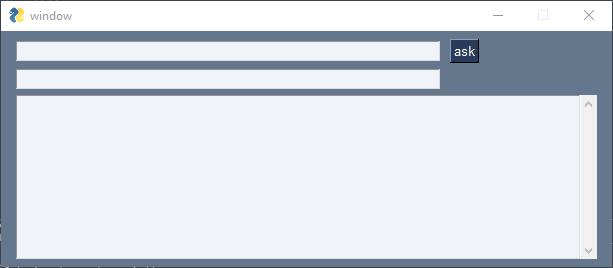
\includegraphics{win.PNG}
		\caption{}
		\label{fig:win}
	\end{figure}
	
	В верхней строке нужно ввести вопрос, на который требуется найти ответ. 
	
	
	\begin{figure}[H]
		\centering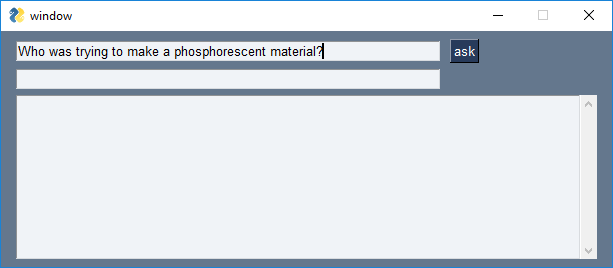
\includegraphics{q11.PNG}
		\caption{}
		\label{fig:ask}
	\end{figure}

	Для того, чтобы задать вопрос, нужно нажать на кнопку "ask" . 
	
	\begin{figure}[H]
		\centering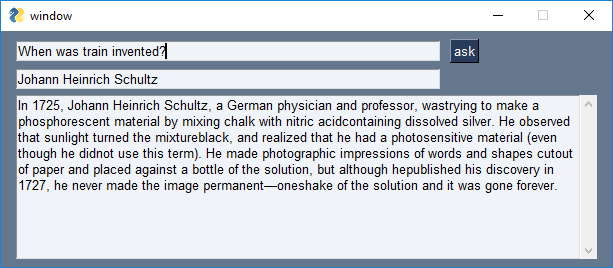
\includegraphics{q1.PNG}
		\caption{}
		\label{fig:get}
	\end{figure}
	
	К сожалению, система не всегда способна найти ответ. Она хорошо работает на фактической информации (например, "Когда был изобретен паровоз?"). Дает ответы на вопросы очень долго, вероятно, из-за огромного размера исходного документа.
	
	\chapter{Выводы}
	
	В рамках данной курсовой работы были исследованы принципы работы вопросно-ответных систем. Реализовано пользовательское приложение в формате диалога на английском языке. В ходе тестирования были обнаружены вопросы, на которые система дает неправильные ответы, также было обнаружено, что из-за огромного размера источника система дает ответы за продолжительное время.
	
	\chapter{Приложение А}
	
	\section{Код программы}
	
\begin{verbatim}
import pandas as pd
import PySimpleGUI as sg
from ast import literal_eval

from cdqa.utils.converters import pdf_converter
from cdqa.utils.filters import filter_paragraphs
from cdqa.utils.download import download_model, download_bnpp_data
from cdqa.pipeline.cdqa_sklearn import QAPipeline

download_model(model='bert-squad_1.1', dir='./models')
df = pdf_converter(directory_path='./data/pdf/')
df.head()
df.to_csv('history_book.csv', index = False)
cdqa_pipeline = QAPipeline(reader='models/bert_qa.joblib')
print('fitting')
cdqa_pipeline.fit_retriever(df)
print('fit')


layout = []
layout.append([sg.InputText(key='t', size=(60, 1)), sg.Button('ask', key='b')])
layout.append([sg.InputText(key='a', size=(60, 1))])
layout.append([sg.Multiline(key='c', size=(80, 10))])
#layout.append([sg.Multiline(key='m', size=(50, 10))])
window = sg.Window('window', layout)
while True:
event, values = window.read()
    if event != 'b':
        break

query = values['t']
prediction = cdqa_pipeline.predict(query)
window['a'].update(prediction[0])
window['c'].update(prediction[2])

\end{verbatim}


	
	
	
\end{document}


